\documentclass[11pt]{article}
\usepackage[margin=1in]{geometry}
\usepackage{amsmath,amssymb,mathtools,bm}
\usepackage{microtype}
\usepackage[T1]{fontenc}
\usepackage{lmodern}
\usepackage{booktabs,array,enumitem,caption}
\usepackage{float}
\usepackage{tikz}
\usetikzlibrary{arrows.meta,positioning,calc,decorations.pathreplacing,shapes.geometric}
\usepackage[hidelinks]{hyperref}
\setlist{nosep}
\setlength{\parskip}{0.55em}
\setlength{\parindent}{0pt}

\newcommand{\dd}{\mathrm{d}}
\newcommand{\Mb}{M_{\mathrm{b}}}
\newcommand{\vf}{v_{\mathrm{f}}}
\newcommand{\Td}{T_{\diamond}}
\newcommand{\FH}{\mathbf F_{\!H}}

\title{\textbf{A Qualitative Cosmology under Hysterical Response Theory}\\[0.35em]
\large One aeon from hot electromagnetic infinity to the next,\\
with a galactic formation subplot}
\author{Andrew Bruce Boyd}
\date{Working qualitative formulation --- September 2026}

\begin{document}
\maketitle
\noindent\textit{Computational note.}
Exploratory experiments and paper writing were assisted by generative AI.
This note is intentionally qualitative: it states no new formal theorems for Lean
verification.
Mathematical claims inherited from companion technical papers of this series are
tagged as such; modelling assumptions and physical hypotheses are tagged likewise.

\begin{abstract}
Hysterical Response Theory (HRT) treats the Hysterical force as a residual of an
already-existing interaction under open-system dynamics---not a new messenger.
Taken together, the technical companions of this series assemble a cyclic
cosmological picture: reciprocal conformal matching identifies the remote
electromagnetic future of one aeon with the hot beginning of the next; expansion
cools the radiation; electroweak cooling drives Hysterical criticality, $\mathbb Z_2$
branch selection, and asymmetric baryogenesis; early gravitational response
amplifies baryonic seeds into galaxies; late dilution produces a vacuum-like
attractor; further cooling into deep de~Sitter reopens an infrared electromagnetic
channel whose active phase transition seeds the following aeon.
The cycle boundaries match exactly under the conformal identification.
A parallel galactic subplot records critical gravity, the capacity selection
$Q\gtrsim O(\sqrt{\Mb})$, relaxation to a stable attractor, the spherical-to-oblate
halo sequence, and the late-time size--mass law $R\sim\Mb^{\alpha}$ with
$\alpha=5/12$ under isotropic accretion.
This paper is a narrative map, not a substitute for the technical derivations.
\end{abstract}
\tableofcontents
\newpage

\section{Purpose and reading contract}
\label{sec:purpose}
The technical papers of this series prove local mechanisms: residual response and
criticality~\cite{boyd2026response}; galactic halos and scaling~\cite{boyd2026galactic};
early growth~\cite{boyd2026early}; late acceleration~\cite{boyd2026late}; branch
asymmetry~\cite{boyd2026branch}; electroweak cooling
baryogenesis~\cite{boyd2026cooling}; and an active conformal cyclic
bridge~\cite{boyd2026ccc}.
None of them, alone, tells the story of a whole universe.

This note does that qualitatively.
It does not re-prove theorems.
It arranges inherited results into one chronological picture of an aeon, then of a
galaxy inside that aeon, with explicit timelines.
Wherever a step is a modelling closure, a physical hypothesis, or an open dynamical
problem, that status is named.

\begin{center}
\small
\begin{tabular}{@{}>{\bfseries}p{0.22\linewidth}p{0.70\linewidth}@{}}
\toprule
Inherited theorem & Result proved in a companion technical paper.\\
Modelling closure & Ansatz needed to connect theorems into cosmology.\\
Physical hypothesis & Claim about Nature, not forced by the maths.\\
Open / not claimed & Saturation amplitudes, abundances, ``Nature is HCCC,'' \ldots\\
\bottomrule
\end{tabular}
\end{center}

\section{One-sentence ontology}
\label{sec:ontology}
Write the observed force as
\begin{equation}
\label{eq:FH}
\boxed{\mathbf F_{\mathrm{observed}}=\mathbf F_{\mathrm{ordinary}}+\FH,}
\qquad
\FH=-\operatorname{Tr}\!\bigl(F\,\mathcal L^{-1}\mathcal S\bigr)
\end{equation}
whenever the resolvent is defined on the relevant stable response
subspace~\cite{boyd2026response}.
No new force carrier is introduced: $\FH$ is a residual component of an
already-existing interaction.
Gravity, electroweak dynamics, and electromagnetism each carry their own residual;
which channel is supercritical depends on epoch and dilution.

\section{The Hysterical aeon at a glance}
\label{sec:cycle-glance}
One cycle of Hysterical Conformal Cyclic Cosmology (HCCC)~\cite{boyd2026ccc}
reads, schematically,
\begin{equation}
\label{eq:cycle}
\boxed{\begin{aligned}
&T=\infty\ \text{(hot EM / radiation)}\\
&\longrightarrow\ \text{expansion cooling}\\
&\longrightarrow\ \text{symmetry breaking / branch selection}\\
&\longrightarrow\ \text{asymmetric baryogenesis}\\
&\longrightarrow\ \text{early galactic formation}\\
&\longrightarrow\ \text{cosmological-constant attractor}\\
&\longrightarrow\ \text{further cooling into de~Sitter}\\
&\longrightarrow\ \text{IR EM Hysterical criticality}\\
&\longrightarrow\ T=\infty\ \text{(next aeon)}.
\end{aligned}}
\end{equation}
The first and last entries are the \emph{same} geometric object under reciprocal
conformal matching: the cold electromagnetic future of one aeon is the hot
electromagnetic beginning of the next~\cite{boyd2026ccc,Penrose2010,Penrose2013CCC}.
The boundaries match exactly.

\begin{figure}[ht]
\centering
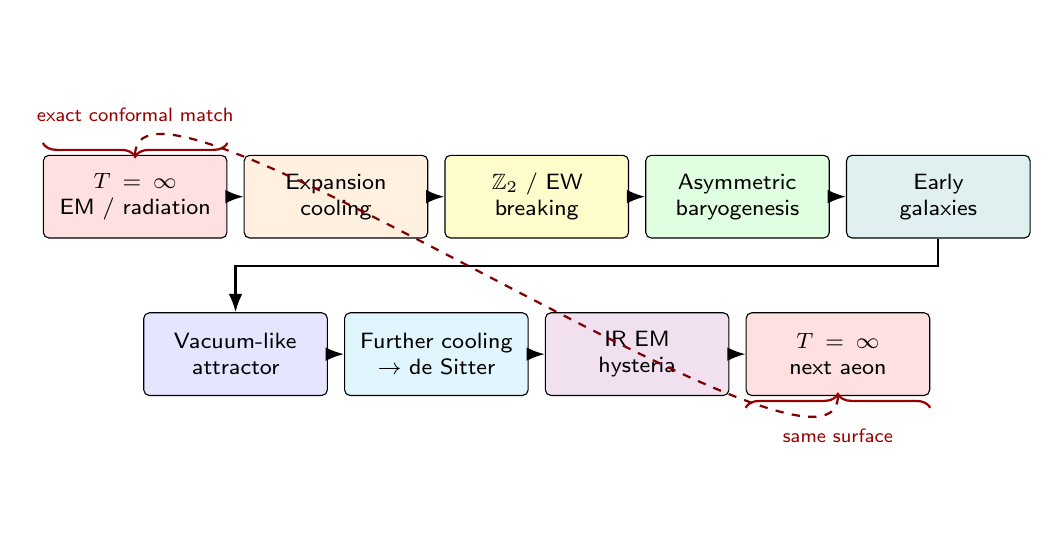
\begin{tikzpicture}[
  font=\small,
  node distance=0.35cm and 0.55cm,
  box/.style={draw, rounded corners=2pt, align=center, inner sep=4pt,
    minimum height=1.05cm, text width=2.05cm, font=\footnotesize\sffamily},
  arr/.style={-{Latex}, thick}
]
\def\y{0}
\node[box, fill=red!12] (tinf) at (0,\y) {$T=\infty$\\EM / radiation};
\node[box, fill=orange!12] (cool) at (2.55,\y) {Expansion\\cooling};
\node[box, fill=yellow!20] (sb) at (5.1,\y) {$\mathbb Z_2$ / EW\\breaking};
\node[box, fill=green!12] (bary) at (7.65,\y) {Asymmetric\\baryogenesis};
\node[box, fill=teal!12] (gal) at (10.2,\y) {Early\\galaxies};

\node[box, fill=blue!10] (lam) at (1.275,-2.0) {Vacuum-like\\attractor};
\node[box, fill=cyan!12] (ds) at (3.825,-2.0) {Further cooling\\$\to$ de~Sitter};
\node[box, fill=violet!12] (irem) at (6.375,-2.0) {IR EM\\hysteria};
\node[box, fill=red!12] (tinf2) at (8.925,-2.0) {$T=\infty$\\next aeon};

\draw[arr] (tinf) -- (cool);
\draw[arr] (cool) -- (sb);
\draw[arr] (sb) -- (bary);
\draw[arr] (bary) -- (gal);
\draw[arr] (gal.south) -- ++(0,-0.35) -| (lam.north);
\draw[arr] (lam) -- (ds);
\draw[arr] (ds) -- (irem);
\draw[arr] (irem) -- (tinf2);

% matching brace
\draw[thick, red!60!black, decorate, decoration={brace,amplitude=5pt,mirror}]
  ($(tinf.north west)+(0,0.15)$) -- ($(tinf.north east)+(0,0.15)$)
  node[midway, above=4pt, font=\scriptsize\sffamily, text=red!60!black]
  {exact conformal match};
\draw[thick, red!60!black, decorate, decoration={brace,amplitude=5pt}]
  ($(tinf2.south west)+(0,-0.15)$) -- ($(tinf2.south east)+(0,-0.15)$)
  node[midway, below=4pt, font=\scriptsize\sffamily, text=red!60!black]
  {same surface};
\draw[red!50!black, dashed, thick] (tinf.north) .. controls +(0,1.6) and +(0,-1.6) .. (tinf2.south);
\end{tikzpicture}
\caption{One Hysterical aeon as a closed loop.
The red dashed identification equates the outgoing $T=\infty$ electromagnetic
future with the incoming $T=\infty$ of the next cycle.}
\label{fig:cycle-loop}
\end{figure}

\section{Aeon timeline (logarithmic cosmic time)}
\label{sec:aeon-timeline}
Figure~\ref{fig:aeon-timeline} places the same stages on a schematic logarithmic
clock inside one aeon.
Times are order-of-magnitude anchors from the technical companions and standard
cosmology, not a fitted chronology of Nature.

\begin{figure}[ht]
\centering
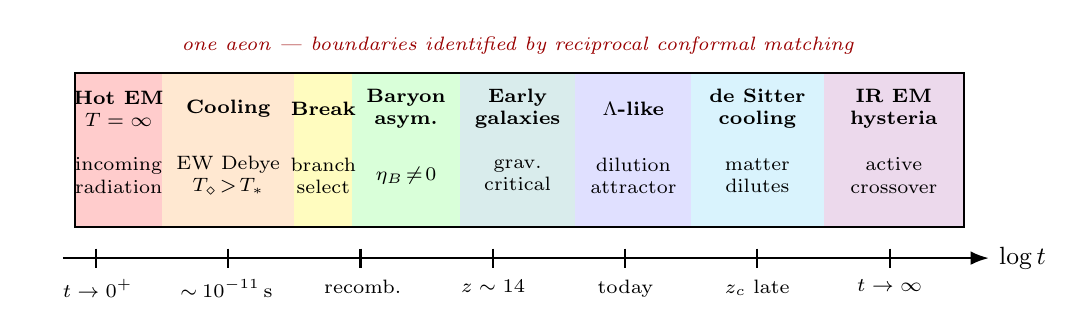
\begin{tikzpicture}[x=1.05cm,y=1cm, font=\sffamily]
% axis
\draw[-{Latex}, thick] (0,0) -- (11.2,0) node[right, font=\small] {$\log t$};
\foreach \x/\lab in {
  0.4/{$t\!\to\!0^+$},
  2.0/{$\!\sim\!10^{-11}\,\mathrm{s}$},
  3.6/{recomb.},
  5.2/{$z\!\sim\!14$},
  6.8/{today},
  8.4/{$z_c$ late},
  10.0/{$t\!\to\!\infty$}
}{
  \draw[thick] (\x,0.12) -- (\x,-0.12);
  \node[below, font=\scriptsize, align=center, text width=1.5cm] at (\x,-0.15) {\lab};
}

% epoch bands
\fill[red!20] (0.15,0.4) rectangle (1.2,2.35);
\fill[orange!18] (1.2,0.4) rectangle (2.8,2.35);
\fill[yellow!25] (2.8,0.4) rectangle (3.5,2.35);
\fill[green!15] (3.5,0.4) rectangle (4.8,2.35);
\fill[teal!15] (4.8,0.4) rectangle (6.2,2.35);
\fill[blue!12] (6.2,0.4) rectangle (7.6,2.35);
\fill[cyan!15] (7.6,0.4) rectangle (9.2,2.35);
\fill[violet!15] (9.2,0.4) rectangle (10.9,2.35);

\draw[thick] (0.15,0.4) rectangle (10.9,2.35);

\node[font=\scriptsize\bfseries, align=center] at (0.675,1.9) {Hot EM\\$T=\infty$};
\node[font=\scriptsize, align=center] at (0.675,1.05) {incoming\\radiation};

\node[font=\scriptsize\bfseries, align=center] at (2.0,1.9) {Cooling};
\node[font=\scriptsize, align=center] at (2.0,1.05) {EW Debye\\$\Td\!>\!T_*$};

\node[font=\scriptsize\bfseries, align=center] at (3.15,1.9) {Break};
\node[font=\scriptsize, align=center] at (3.15,1.05) {branch\\select};

\node[font=\scriptsize\bfseries, align=center] at (4.15,1.9) {Baryon\\asym.};
\node[font=\scriptsize, align=center] at (4.15,1.05) {$\eta_B\!\neq\!0$};

\node[font=\scriptsize\bfseries, align=center] at (5.5,1.9) {Early\\galaxies};
\node[font=\scriptsize, align=center] at (5.5,1.05) {grav.\\critical};

\node[font=\scriptsize\bfseries, align=center] at (6.9,1.9) {$\Lambda$-like};
\node[font=\scriptsize, align=center] at (6.9,1.05) {dilution\\attractor};

\node[font=\scriptsize\bfseries, align=center] at (8.4,1.9) {de~Sitter\\cooling};
\node[font=\scriptsize, align=center] at (8.4,1.05) {matter\\dilutes};

\node[font=\scriptsize\bfseries, align=center] at (10.05,1.9) {IR EM\\hysteria};
\node[font=\scriptsize, align=center] at (10.05,1.05) {active\\crossover};

\node[font=\scriptsize\itshape, text=red!60!black] at (5.5,2.7)
  {one aeon --- boundaries identified by reciprocal conformal matching};
\end{tikzpicture}
\caption{Schematic logarithmic timeline of one Hysterical aeon.
The electroweak concurrency clock $t_\diamond\sim10^{-11}\,\mathrm{s}$ is inherited
from the cooling-baryogenesis companion~\cite{boyd2026cooling,DOnofrio2014};
the $z\sim14$ galactic timing window from the early-universe
companion~\cite{boyd2026early,Carniani2024}; the late vacuum-like attractor from
the late-universe companion~\cite{boyd2026late}; the IR EM crossover from
HCCC~\cite{boyd2026ccc}.}
\label{fig:aeon-timeline}
\end{figure}

\section{Phase-by-phase narrative}
\label{sec:phases}

\subsection{\texorpdfstring{Hot electromagnetic infinity ($T=\infty$)}{Hot electromagnetic infinity}}
Under reciprocal conformal matching with unit reciprocity, outgoing de~Sitter
scale-factor asymptotics map to an incoming radiation-era law
$a\propto t^{1/2}$, and regular conformal Maxwell data that appear cold on the
outgoing side appear hot on the incoming side~\cite{boyd2026ccc}.
That hot branch is the Big-Bang-like content of the new aeon: a radiation-dominated
electromagnetic beginning at formal $T=\infty$.
Whether \emph{our} observed Big Bang was such a crossover is a physical hypothesis,
not a theorem~\cite{boyd2026ccc}.

\subsection{Cooling driven by cosmological expansion}
Expansion redshifts temperatures.
In the electroweak residual channel, Debye reciprocal stiffnesses with fixed
nonzero off-diagonal feedback force a unique criticality temperature
$\Td$: the neutral residual is subcritical for all $T>\Td$ and supercritical for
all $0<T<\Td$~\cite{boyd2026cooling}.
Cooling is therefore not merely a thermodynamic backdrop; it is the driver that
pushes the electroweak Hysterical channel across criticality.

\subsection{Symmetry breaking / branch selection}
Once supercritical, a CP-odd Hysterical collective mode spontaneously breaks a
conjugation $\mathbb Z_2$~\cite{boyd2026branch}.
The two branches are opposite; Nature need not prefer a global sign---our classical
patch simply occupies one branch.
This is spontaneous branch selection, not an externally imposed bias.

\subsection{Asymmetric baryogenesis}
If that odd branch rolls concurrently with active Standard Model $B{+}L$
violation, with a nonzero $YW\widetilde W$ portal and nonempty overlap
$\mathcal C=(T_*,\Td)$ (equivalently $\Td>T_*$), opposite nonzero baryon yields
appear on the two branches~\cite{boyd2026cooling,boyd2026branch}:
\begin{equation}
\eta_B[Y_+]=-\eta_B[Y_-]\neq0.
\end{equation}
Lattice GeV edges convert the concurrent window into
$t_\diamond\sim10^{-11}\,\mathrm{s}$~\cite{boyd2026cooling,DOnofrio2014}.
The observed magnitude $\eta_B\sim10^{-10}$ is not computed in those papers; the
mechanism and analytic concurrency are.

\subsection{Early galactic formation}
After decoupling, a local gravitational response reservoir closed attractively into
dust growth is supercritical under positive matter--response
coupling~\cite{boyd2026early}.
In a Planck-like baryon-only timing suite, a $10^{-5}$ seed can reach nonlinear
contrast by $z\simeq14$ for sufficiently strong coupling---compatible in
\emph{timing} with spectroscopically confirmed JWST galaxies at that
epoch~\cite{boyd2026early,Carniani2024,Planck2018}.
Abundances and stellar masses are not claimed.
The galactic subplot of Section~\ref{sec:galactic} unpacks the mature morphology
that follows.

\subsection{Cosmological-constant attractor}
Homogeneous dilution of a conserved density, together with a relaxation gap that
vanishes as a positive power of that density, forces a unique criticality scale
factor~\cite{boyd2026late}.
Past that scale, a pitchfork attractor and fluid completion produce a positive
asymptotic density with $w\to-1$ from below---a vacuum-like late-universe term
without a new force carrier.
A one-parameter background confrontation with Planck flat $\Lambda$CDM is a shape
test, not a microscopic derivation of the observed magnitude~\cite{boyd2026late,Planck2018}.

\subsection{Further cooling and infrared electromagnetic hysteria}
Charge conservation still forbids creating homogeneous net charge from
neutrality, but finite-wavenumber electromagnetic response remains
allowed~\cite{boyd2026late,boyd2026ccc}.
In deep late-time de~Sitter, a helical electromagnetic--response linearisation is
infrared-first: a finite unstable band of physical wavenumber becomes supercritical
when the response gain exceeds the zero-mode threshold~\cite{boyd2026ccc}.
A modelling completion then pumps finite-$k$ photons.
That active infrared electromagnetic phase transition---not a passive conformal
identification after matter evaporates---is the dynamical heart of HCCC, set against
Penrose's CCC geometry~\cite{boyd2026ccc,Penrose2010,Penrose2013CCC}.

\subsection{\texorpdfstring{Return to $T=\infty$: exact boundary matching}{Return to infinity: exact boundary matching}}
Reciprocal conformal matching with $\Omega_+\Omega_-=C_0$ transports Maxwell data
while densities rescale as $\rho=\Omega^{-4}\hat\rho$.
Finite conformal radiation density is cold outgoing and hot
incoming~\cite{boyd2026ccc}.
Under unit reciprocity, outgoing $a_-\sim 1/(H_-|\eta|)$ becomes incoming
$a_+\propto t_+^{1/2}$.
Thus the cycle closes:
\begin{equation}
\label{eq:match}
\boxed{\text{outgoing }T=\infty\text{ EM future}\ \equiv\ \text{incoming }T=\infty\text{ of the next aeon}.}
\end{equation}
The boundaries match exactly by construction of the conformal identification.
What remains open is dynamical: saturated amplitude, Einstein--Maxwell--response
junction regularity, and thermalisation~\cite{boyd2026ccc}.

\section{Galactic formation subplot}
\label{sec:galactic}
Galaxies are not a separate ontology.
They are the spatial organisation of the \emph{gravitational} Hysterical residual
inside an aeon that already has baryons~\cite{boyd2026galactic,boyd2026response}.

\subsection{Critical gravity}
The response-theory paper classifies closed-loop gravitational response by the
spectral abscissa of the gain Jacobian~\cite{boyd2026response}.
When the cosmological matter--response coupling is positive, the frozen early-universe
Jacobian is supercritical, so the inherited neutrality--instability theorem
applies and growth exceeds ordinary dust~\cite{boyd2026early}.
That is the ``critical gravity'' stage of assembly: small baryonic seeds are
amplified by a persistent residual sector without importing a cold-dark-matter
perturbative scaffold (timing claim, not abundance claim).

\subsection{\texorpdfstring{Capacity selection $Q\gtrsim O(\sqrt{\Mb})$}{Capacity selection}}
Let $Q$ be the total residual-production rate of the ballistic halo and $\Mb$ the
baryonic mass.
Formation and mature retention are conjectured to require response capacity at
least of square-root order~\cite{boyd2026galactic}:
\begin{equation}
\label{eq:capacity}
\boxed{Q\gtrsim O\bigl(\sqrt{\Mb}\bigr)}.
\end{equation}
This is a selection rule, not a transport theorem.
Separately, given a capacity--filling ODE, mature systems are driven to a stable
attractor $Q^{2}\propto\Mb$ (theorem/corollary of that setup), which with flat
response rotation $\vf^{2}=CQ$ yields the baryonic Tully--Fisher exponent
$\vf^{4}\propto\Mb$~\cite{boyd2026galactic,mcgaugh2012}.

\subsection{Relaxation and stability}
Response-limited assembly is modelled by a logistic filling dynamics with a stable
fixed point $y_*\in(0,1]$~\cite{boyd2026galactic}.
Systems that satisfy~\eqref{eq:capacity} relax onto the square-root attractor;
systems that cannot maintain capacity are not expected to remain as mature
response-supported galaxies.
Stability here is ordinary ODE stability of the filling fixed point, not a claim
of absolute cosmic permanence.

\subsection{Spherical halo to oblate}
The leading ballistic far-field residual density is spherical,
$n=Q/(4\pi v r^{2})+O(r^{-4})$, even when the baryonic source is
flattened~\cite{boyd2026galactic}.
The first surviving angular correction for a planar source is a response quadrupole
of oblate sign under the same linear Poisson closure, with effective flattening
$q_{\mathrm{eff}}^{-2}(R)=1+s/R^{2}+O(R^{-4})$~\cite{boyd2026galactic}.
Morphologically: assemble a spherical response halo first; retain source shape in
subleading multipoles that become the asymptotic oblate correction.

\subsection{\texorpdfstring{Size--mass law $R\sim M_b^{\alpha}$}{Size-mass law}}
Under isotropic accretion from a homogeneous intergalactic reservoir, virial
specific angular momentum $j\propto\Mb^{2/3}$, and size proxy $R\sim j/\vf$, the
mature BTFR attractor implies~\cite{boyd2026galactic}
\begin{equation}
\label{eq:size-mass}
\boxed{R\propto\Mb^{5/12}},
\qquad\text{i.e.}\quad\alpha=\tfrac{5}{12}.
\end{equation}
Anisotropic or filamentary accretion would change $\alpha$.
The exponent is comparable to the steeper end of observed late-type size--mass
slopes; it is a conditional scaling prediction, not a universal fit.

\begin{figure}[H]
\centering
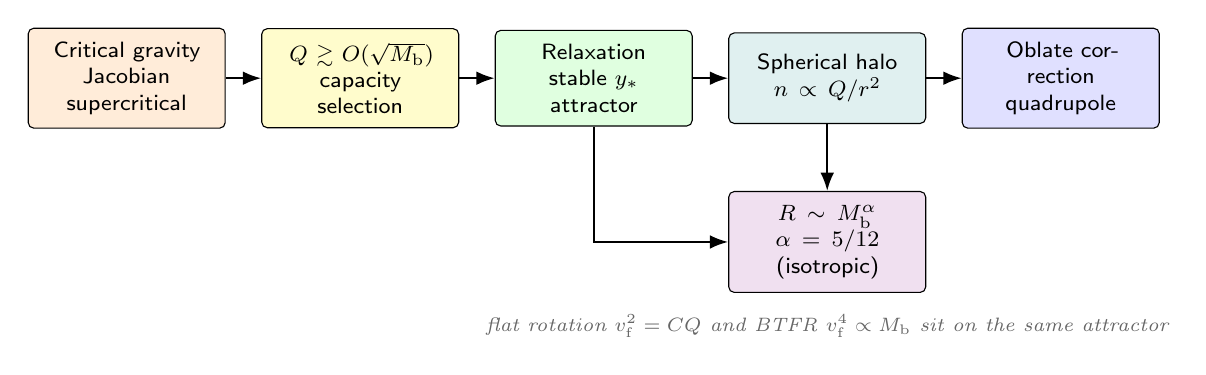
\begin{tikzpicture}[
  font=\sffamily\footnotesize,
  stage/.style={draw, rounded corners=2pt, align=center, inner sep=5pt,
    minimum height=1.15cm, text width=2.15cm},
  arr/.style={-{Latex}, thick}
]
\node[stage, fill=orange!15] (crit) {Critical gravity\\Jacobian supercritical};
\node[stage, fill=yellow!20, right=0.45cm of crit] (cap) {$Q\gtrsim O(\sqrt{\Mb})$\\capacity selection};
\node[stage, fill=green!12, right=0.45cm of cap] (rel) {Relaxation\\stable $y_*$ attractor};
\node[stage, fill=teal!12, right=0.45cm of rel] (sph) {Spherical halo\\$n\propto Q/r^{2}$};
\node[stage, fill=blue!12, right=0.45cm of sph] (obl) {Oblate correction\\quadrupole};
\node[stage, fill=violet!12, below=0.85cm of sph] (size) {$R\sim\Mb^{\alpha}$\\$\alpha=5/12$ (isotropic)};

\draw[arr] (crit) -- (cap);
\draw[arr] (cap) -- (rel);
\draw[arr] (rel) -- (sph);
\draw[arr] (sph) -- (obl);
\draw[arr] (rel.south) |- (size.west);
\draw[arr] (sph.south) -- (size.north);

\node[font=\scriptsize\itshape, text=black!60, below=0.15cm of size]
  {flat rotation $\vf^{2}=CQ$ and BTFR $\vf^{4}\propto\Mb$ sit on the same attractor};
\end{tikzpicture}
\caption{Galactic formation subplot: from critical gravitational response to
mature morphology and size--mass scaling.}
\label{fig:galactic-flow}
\end{figure}

\begin{figure}[H]
\centering
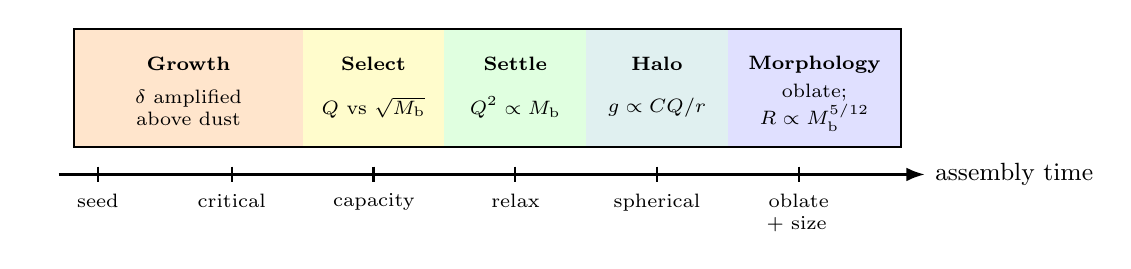
\begin{tikzpicture}[x=1.0cm, y=1cm, font=\sffamily]
\draw[-{Latex}, thick] (0,0) -- (11.0,0) node[right, font=\small] {assembly time};
\foreach \x/\lab in {
  0.5/{seed},
  2.2/{critical},
  4.0/{capacity},
  5.8/{relax},
  7.6/{spherical},
  9.4/{oblate + size}
}{
  \draw[thick] (\x,0.1) -- (\x,-0.1);
  \node[below, font=\scriptsize, align=center, text width=1.55cm] at (\x,-0.12) {\lab};
}
\fill[orange!20] (0.2,0.35) rectangle (3.1,1.85);
\fill[yellow!20] (3.1,0.35) rectangle (4.9,1.85);
\fill[green!12] (4.9,0.35) rectangle (6.7,1.85);
\fill[teal!12] (6.7,0.35) rectangle (8.5,1.85);
\fill[blue!12] (8.5,0.35) rectangle (10.7,1.85);
\draw[thick] (0.2,0.35) rectangle (10.7,1.85);

\node[font=\scriptsize\bfseries, align=center] at (1.65,1.4) {Growth};
\node[font=\scriptsize, align=center] at (1.65,0.85) {$\delta$ amplified\\above dust};

\node[font=\scriptsize\bfseries, align=center] at (4.0,1.4) {Select};
\node[font=\scriptsize, align=center] at (4.0,0.85) {$Q$ vs $\sqrt{\Mb}$};

\node[font=\scriptsize\bfseries, align=center] at (5.8,1.4) {Settle};
\node[font=\scriptsize, align=center] at (5.8,0.85) {$Q^{2}\propto\Mb$};

\node[font=\scriptsize\bfseries, align=center] at (7.6,1.4) {Halo};
\node[font=\scriptsize, align=center] at (7.6,0.85) {$g\propto CQ/r$};

\node[font=\scriptsize\bfseries, align=center] at (9.6,1.4) {Morphology};
\node[font=\scriptsize, align=center] at (9.6,0.85) {oblate;\\$R\propto\Mb^{5/12}$};
\end{tikzpicture}
\caption{Schematic galactic assembly timeline (not to absolute cosmic scale).
Early nonlinearity by $z\sim14$ is a timing window from the early-universe
companion; capacity, attractor, halo, and oblate/size--mass structure are from
galactic modelling.}
\label{fig:galactic-timeline}
\end{figure}

\section{Two clocks, one ontology}
\label{sec:two-clocks}
It helps to keep two clocks distinct:
\begin{center}
\small
\begin{tabular}{@{}>{\bfseries}p{0.28\linewidth}p{0.64\linewidth}@{}}
\toprule
Aeon clock & Cosmic expansion, cooling, EW concurrency, late dilution, IR EM crossover.\\
Galactic clock & Local criticality, capacity, relaxation, halo morphology, size--mass.\\
\midrule
Shared ontology & Both are residual responses of already-existing interactions
(electroweak / electromagnetic / gravitational), not new carriers.\\
\bottomrule
\end{tabular}
\end{center}
The galactic subplot lives \emph{inside} the aeon timeline, after baryons exist and
before (and during) the late vacuum-like era.
It does not interrupt the cycle; it populates it.

\section{What is and is not claimed}
\label{sec:status}
\begin{center}
\small
\begin{tabular}{@{}p{0.48\linewidth}p{0.44\linewidth}@{}}
\toprule
\textbf{Narrative element} & \textbf{Status}\\
\midrule
Residual ontology~\eqref{eq:FH} & Inherited~\cite{boyd2026response}.\\
Hot/cold conformal match; dS$\to$radiation & Inherited theorems~\cite{boyd2026ccc}.\\
Exact cycle-boundary identification & Modelling/geometry of HCCC + CCC spine.\\
EW cooling $\Rightarrow$ unique $\Td$ & Inherited~\cite{boyd2026cooling}.\\
$\mathbb Z_2$ branch asymmetry $\Rightarrow\eta_B$ & Inherited, concurrency assumed~\cite{boyd2026branch,boyd2026cooling}.\\
Observed $\eta_B\sim10^{-10}$ & Not derived.\\
Early $z\sim14$ nonlinearity timing & Numerical experiments~\cite{boyd2026early}.\\
Galaxy abundances / stellar masses & Not claimed.\\
$Q\gtrsim O(\sqrt{\Mb})$ & Formation conjecture~\cite{boyd2026galactic}.\\
$Q^{2}\propto\Mb$, BTFR, $R\propto\Mb^{5/12}$, oblate & Inherited (with stated assumptions)~\cite{boyd2026galactic}.\\
Late vacuum-like attractor & Inherited~\cite{boyd2026late}.\\
IR EM unstable band / photon pump & Theorems + modelling~\cite{boyd2026ccc}.\\
Saturation, junction, thermalisation & Open~\cite{boyd2026ccc}.\\
``Nature realises this whole cycle'' & Physical hypothesis; not claimed as theorem.\\
\bottomrule
\end{tabular}
\end{center}

\section{Closing picture}
\label{sec:close}
Under Hysterical Response Theory the universe is cyclic, but not passively so.
Each aeon begins as hot electromagnetic radiation identified with the conformal
future of its predecessor; cools through electroweak branch selection and
baryogenesis; grows galaxies from gravitational residual criticality under the
capacity rule $Q\gtrsim O(\sqrt{\Mb})$; settles into a vacuum-like attractor; and
ends when infrared electromagnetic hysteria actively reseeds the next hot infinity.
The boundaries match exactly.
Galaxies inside the cycle relax from spherical response halos toward oblate
corrections with $R\sim\Mb^{5/12}$ under isotropic accretion.

This qualitative map is meant to be readable in one sitting.
The mathematics lives in the companions cited above.

\bibliographystyle{plain}
\bibliography{paper_refs}
\end{document}
